\chapter{Results and Analysis}
\phantomsection
\label{ch:results}

\section{Text Detection Results}
\label{sec:detection-results}

The text detection model, based on the CRAFT (Character Region Awareness for Text detection) 
architecture, was evaluated on a test set consisting of 20 images. The model achieved an impressive 
Intersection over Union (IoU) score of 0.98 when compared to the ground truth annotations, 
demonstrating high accuracy in detecting text regions.

The training process was conducted on a dataset of 175 images, with an additional 20 images 
used for validation. The evaluation results indicate that the model is capable of accurately 
detecting text in all test images, showcasing its generalization ability and robustness across 
various text-containing scenes.

\begin{figure}[ht]
    \centering
    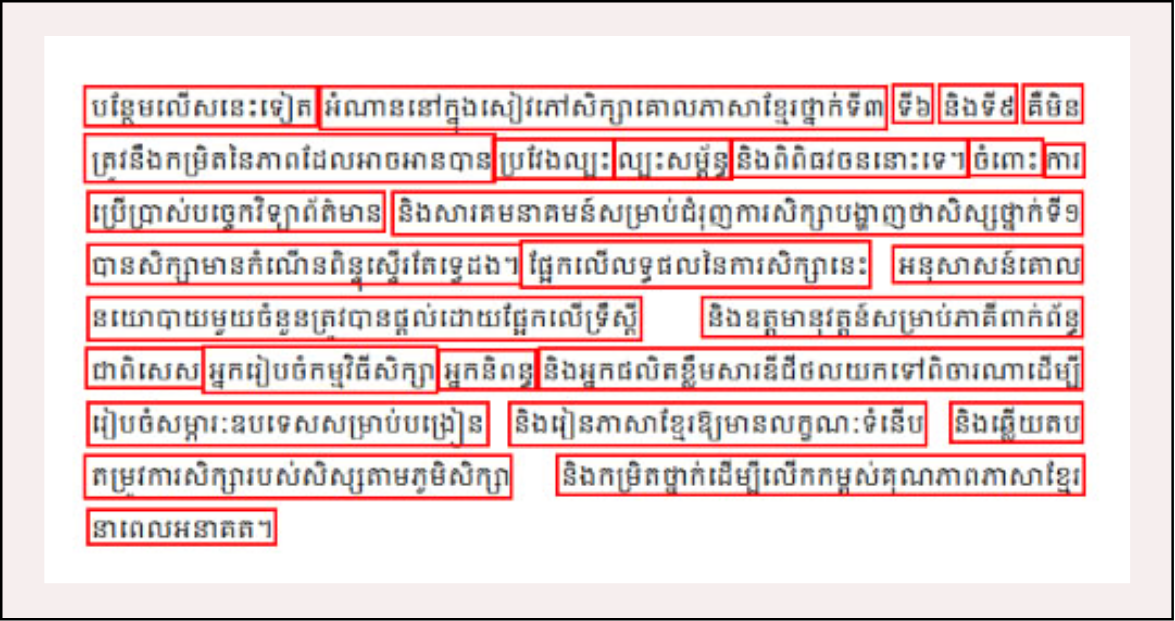
\includegraphics[width=1\textwidth]{figures/image_detection_craft_01.png}
    \caption{Testing with documentation image type: example of text detection using the CRAFT 
    model on a natural scene text image.}
    \label{fig:detection-craft}
\end{figure}

The results from testing with clean text from documentation images are shown in Figure 
\ref{fig:detection-craft}. The model is able to detect text in each sentence, 
even when the text is separated by spaces. This is important for the OCR model to 
work with short text sentences, as it is able to recognize the text more accurately. 
For example, if the model is given the text "This is a test", it should be able to 
detect each word as a single entity, rather than as whole sentence. 
By detecting text in this way, the model is able to recognize the text 
more accurately.

\begin{figure}[ht]
    \centering
    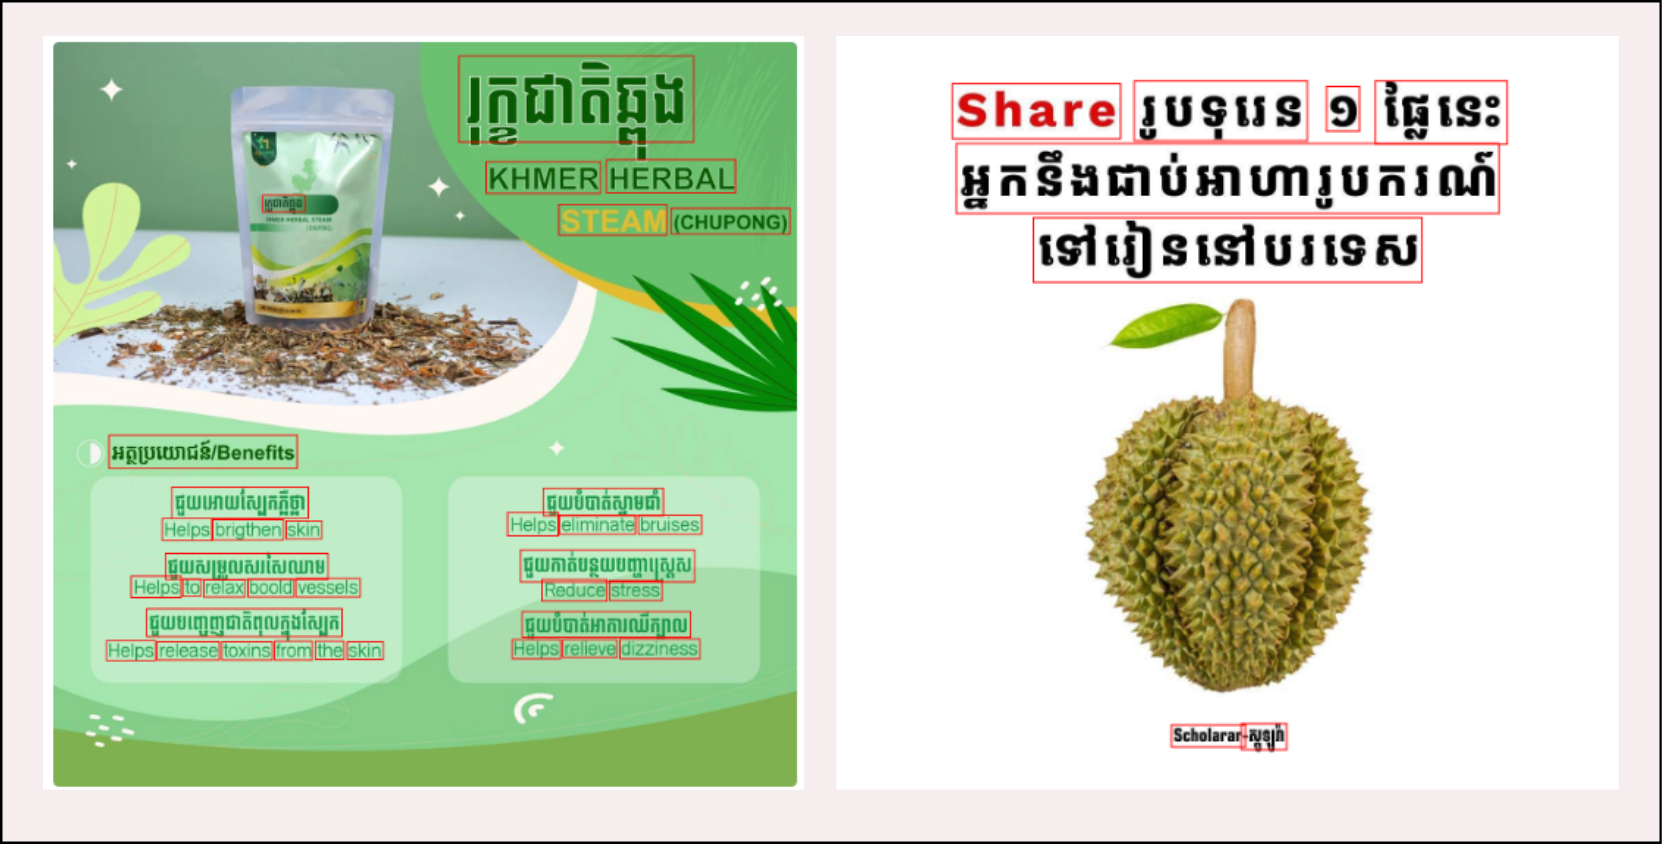
\includegraphics[width=1\textwidth]{figures/image_detection_craft_02.png}
    \caption{Testing with post image type and complex scenes: example of text detection using the CRAFT 
    model on a natural scene text image.}
    \label{fig:detection-craft-post}
\end{figure}

As you can see from the example in Figure \ref{fig:detection-craft-post}, 
the model is able to detect text even when it is very small, such as the text on the poster. 
This demonstrates the model's robustness and ability to detect text in a variety of contexts and scenarios.
\section{Text Recognition Results}
\label{sec:recognition-results}
The text recognition model, based on the TrOCR (Transformer-based OCR) architecture, was
evaluated on a test set consisting of real dataset manually collected amount 3000 images, we
spend time around 3 days to collect this dataset for fairly evaluation. The testing dataset
containing such as char by char, word by word, and sentence by sentence, it's also included
both languages, Khmer and English. The model achieved an impressive result, we achieved CER
( Character Error Rate) of 0.05 and WER (Word Error Rate) of 0.03, demonstrating high accuracy
in recognizing text in the images.
\section{Error Analysis and Failure Cases}
\label{sec:error-analysis}
Systematic analysis of common error patterns and challenging cases that lead to recognition failures.

\section{System Robustness and Generalization}
\label{sec:robustness}
Evaluation of the system's ability to generalize across different document types, fonts, and image quality conditions.
